\section{XSeparation Compiler}
\label{sec:compilation}
%XSeparation generates object-oriented code containing additional constructs for bidirectional traceability. Hence, a compilation process is needed to transform the XSeparation-generated code into machine code.
This section presents the architecture of the XSeparation compiler. %to transform the XSeparation-generated code into machine code.
\begin{figure}
	\centering
	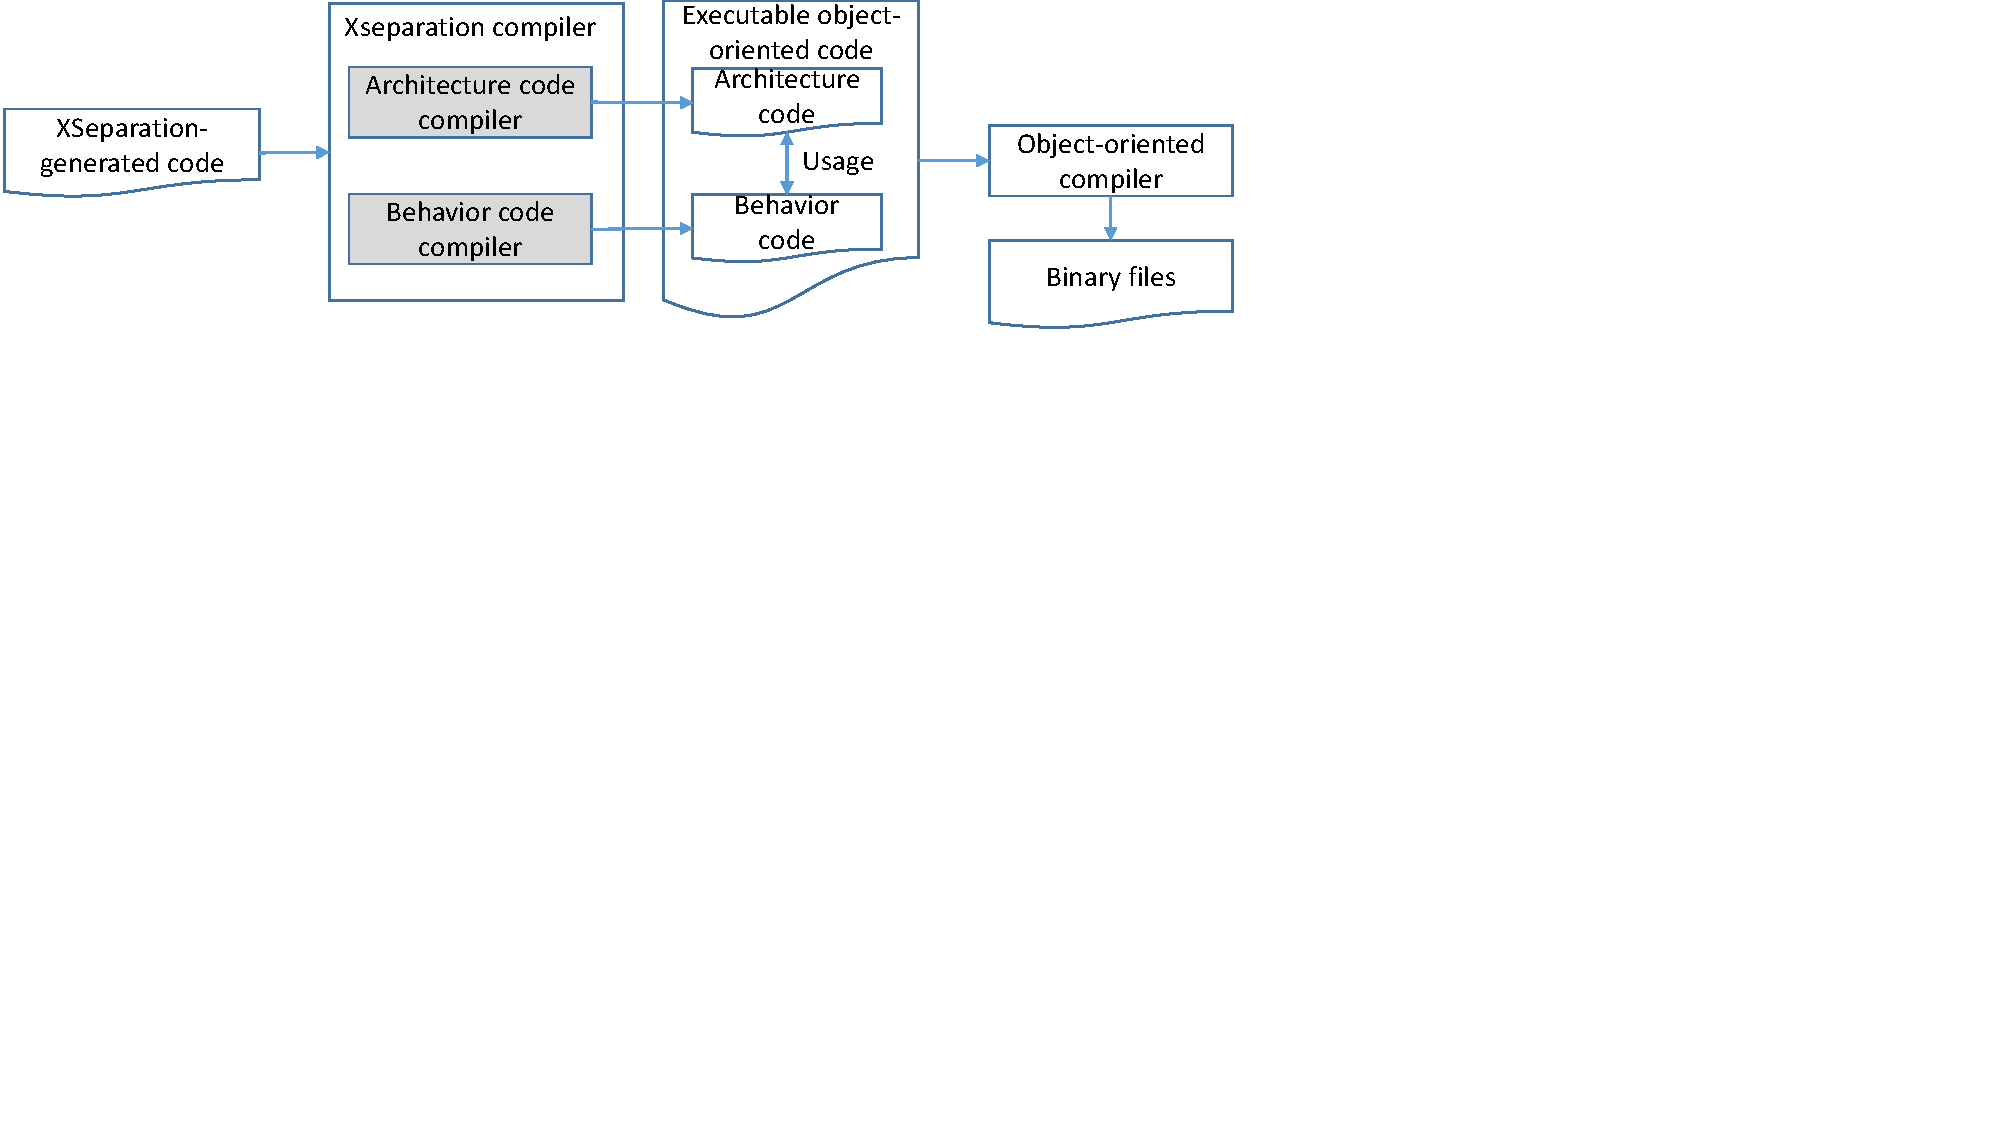
\includegraphics[clip, trim=0cm 13.3cm 12.8cm 0cm, width=\columnwidth]{figures/compilerarchitecture.pdf}
	\caption{XSeparation compiler's architecture} 
	\label{fig:compilerarchitecture}
\end{figure}
Fig. \ref{fig:compilerarchitecture} shows the compilation process, which takes as input the XSeparation-generated code, and produces the binary files by three two steps: \textcircled{1} generation of executable object-oriented code by the XSeparation compiler from XSeparation-generated code; \textcircled{2} production of binary files from the executable code by using object-oriented compilers such as GCC for C++ and Javac for Java.

The XSeparation compiler consists of two grayed sub-modules: \tb{Structure code compiler}, which takes as input the \tb{Component structure-prescribed code}, \tb{User-filled skeleton code}, and \tb{Component structure-provided implementation code} parts to produce \tb{Structure code}, while \tb{Behavior code compiler} takes as input the other parts to generate \tb{Behavior code}. 



\vskip 0.1cm
\noindent
\tb{Structure code compiler:}
Listing \ref{lst:archcodecompiler} shows an executable \tb{Structure code} segment generated for the \ttt{System} example using ports with interfaces.
Each port is generated to a pointer attribute (lines 12 and 15) while each part to an object attribute (lines 3,4,5).
A configuration is transformed into a method named \ttt{configuration}.
When a method is called through a port as in Listing \ref{lst:producerinteraction}, for example \ttt{push} through the \ttt{pPush} port, the corresponding method implemented in FIFO is invoked. 

\begin{figure}
\begin{minipage}{0.95\columnwidth}
	\lstinputlisting[language=C++, caption={Executable code generated by XSeparation compiler for the structure of \ttt{System}}, label=lst:archcodecompiler,frame=f]{code/archcodecompiler.cpp}
\end{minipage} 
\end{figure}

\vskip 0.1cm
\noindent
\tb{Behavior code compiler:}
It generates executable code from the \tb{Behavior-prescribed code} and \tb{State machine action code} similarly to code generation approaches from UML State Machines in MDE tools such as Rhapsody and Sinelabore \cite{sinelabore}.
However, only a subset of UML State Machine concepts is supported by these tools, e.g. Rhapsody does not support junctions, and truly concurrent execution of orthogonal regions
\cite{ibmdiff} (see \cite{specification_uml_2007} for more detail) and the support for pseudo states such as history, choice and junction is poor \cite{EA, sinelabore}. 
%The concurrency of the orthogonal regions is often implemented sequentially \cite{Badreddin2014}. 
%In addition, there are other issues such as event processing speed, executable file size, and UML semantic-conformance defined by a recent work on the Precise Semantics of State Machine (PSSM) \cite{OMG2015}.
XSeparation compiler supports full features of state machines.
Due to space limitation, the details of patterns and evaluation for state machine code generation are not presented in this paper.



In the next section, XSeparation will be implemented as an extension of the Papyrus modeling tool and evaluated by developing a case study of software application for LEGO.